\section{Model Configuration Details}
\label{appendix:config}

This appendix provides detailed configuration specifications and implementation details for both \supra{} and \zennano{} models.

\subsection{Complete Model Specifications}

\subsubsection{Base Model Architecture}

\begin{table}[H]
\centering
\begin{tabular}{lr}
\toprule
\textbf{Parameter} & \textbf{Value} \\
\midrule
Architecture & Transformer Decoder \\
Model Dimension ($d_{model}$) & 2048 \\
Feed-forward Dimension ($d_{ff}$) & 11008 \\
Number of Layers & 40 \\
Number of Attention Heads & 16 \\
Head Dimension ($d_k$) & 128 \\
Number of KV Heads & 16 \\
Vocabulary Size & 151,936 \\
Maximum Sequence Length & 32,768 \\
Positional Encoding & RoPE (base=10000) \\
Activation Function & SwiGLU \\
Layer Normalization & RMSNorm \\
Dropout Rate & 0.0 \\
Attention Dropout & 0.0 \\
Total Parameters & 3,950,000,000 \\
\bottomrule
\end{tabular}
\caption{Complete base model specifications}
\label{tab:complete-specs}
\end{table}

\subsubsection{LoRA Configuration Details}

\begin{table}[H]
\centering
\begin{tabular}{lcc}
\toprule
\textbf{Parameter} & \textbf{\supra{}} & \textbf{\zennano{}} \\
\midrule
LoRA Rank ($r$) & 8 & 8 \\
LoRA Alpha ($\alpha$) & 16 & 16 \\
LoRA Dropout & 0.1 & 0.1 \\
Target Modules & q\_proj, k\_proj, v\_proj, o\_proj & q\_proj, k\_proj, v\_proj, o\_proj \\
Scaling Factor & $\alpha/r = 2.0$ & $\alpha/r = 2.0$ \\
Trainable Parameters & 26,738,688 & 26,738,688 \\
Percentage of Total & 0.67\% & 0.67\% \\
\bottomrule
\end{tabular}
\caption{LoRA configuration for both models}
\label{tab:lora-config}
\end{table}

\subsection{Training Hyperparameters}

\subsubsection{Optimizer Configuration}

\begin{lstlisting}[caption=Complete training configuration,label=lst:training-config]
# Supra Nexus o1 Configuration
supra_config = {
    "model_name": "base-models/Qwen3-4B-2507-Thinking-2507-MLX-8bit",
    "train_data": "training/mlx_thinking_train.jsonl",
    "valid_data": "training/mlx_thinking_valid.jsonl",
    "adapter_path": "adapters/supra-nexus-o1-thinking",
    
    # Training parameters
    "batch_size": 1,
    "learning_rate": 5e-5,
    "num_iters": 100,
    "steps_per_report": 10,
    "steps_per_eval": 25,
    "resume_adapter_file": None,
    "adapter_path": "adapters/supra-nexus-o1-thinking",
    "save_every": 25,
    "test": False,
    "test_batches": 100,
    
    # LoRA parameters
    "lora_layers": 16,
    "lora_rank": 8,
    "lora_alpha": 16,
    "lora_dropout": 0.1,
    
    # Optimization
    "grad_accumulation_steps": 2,
    "max_seq_length": 512,
    "warmup_steps": 10,
    "weight_decay": 0.01,
    "grad_clip": 1.0,
    
    # MLX specific
    "seed": 42,
    "mixed_precision": True
}

# Zen Nano Configuration  
zen_config = {
    "model_name": "base-models/Qwen3-4B-2507-Instruct-2507-MLX-8bit", 
    "train_data": "training/mlx_instruct_train.jsonl",
    "valid_data": "training/mlx_instruct_valid.jsonl",
    "adapter_path": "adapters/supra-nexus-o1-instruct",
    
    # Training parameters (different learning rate)
    "batch_size": 1,
    "learning_rate": 3e-5,  # Lower for instruct model
    "num_iters": 100,
    "steps_per_report": 10,
    "steps_per_eval": 25,
    
    # Same LoRA and optimization settings as Supra
    **{k: v for k, v in supra_config.items() 
       if k.startswith(('lora_', 'grad_', 'max_', 'warmup', 'weight', 'seed', 'mixed'))}
}
\end{lstlisting}

\subsection{Data Format Specifications}

\subsubsection{Training Data Schema}

\begin{lstlisting}[caption=JSON schema for training data,label=lst:data-schema]
{
  "$schema": "http://json-schema.org/draft-07/schema#",
  "type": "object",
  "properties": {
    "messages": {
      "type": "array",
      "items": {
        "type": "object",
        "properties": {
          "role": {
            "type": "string",
            "enum": ["user", "assistant", "system"]
          },
          "content": {
            "type": "string",
            "minLength": 1
          }
        },
        "required": ["role", "content"]
      },
      "minItems": 2
    }
  },
  "required": ["messages"]
}
\end{lstlisting}

\subsubsection{Thinking Tag Structure}

For \supra{} training data, the thinking tag structure follows this pattern:

\begin{lstlisting}[caption=Thinking tag structure specification,label=lst:thinking-structure]
# General structure
<thinking>
[Internal reasoning process]
- Problem analysis
- Step-by-step solution development  
- Intermediate calculations or logic
- Verification of results
- Alternative approaches considered
</thinking>

[Final formatted response]

# Example patterns:
## Mathematical problems:
<thinking>
Let me break down this problem:
1. Identify what's being asked
2. List given information
3. Choose appropriate method
4. Work through calculations
5. Verify the answer
</thinking>

## Logic problems:
<thinking>
I need to analyze this systematically:
- What are the premises?
- What logical rules apply?
- What can I deduce step by step?
- Are there any contradictions?
- What's the logical conclusion?
</thinking>

## Code problems:
<thinking>
To solve this coding problem:
1. Understand the requirements
2. Consider edge cases
3. Choose appropriate algorithms/data structures
4. Write the implementation
5. Test with examples
</thinking>
\end{lstlisting}

\subsection{Evaluation Metrics and Benchmarks}

\subsubsection{Custom Reasoning Quality Metrics}

We developed several custom metrics for evaluating reasoning quality:

\begin{table}[H]
\centering
\begin{tabular}{lp{8cm}c}
\toprule
\textbf{Metric} & \textbf{Description} & \textbf{Scale} \\
\midrule
Step Clarity & How clearly each reasoning step is explained & 1-5 \\
Logical Flow & Coherence and logical progression of reasoning & 1-5 \\
Completeness & Whether all necessary steps are included & 1-5 \\
Accuracy & Correctness of intermediate and final results & 1-5 \\
Verification & Presence and quality of answer verification & 1-5 \\
Educational Value & How well the reasoning teaches the method & 1-5 \\
\bottomrule
\end{tabular}
\caption{Custom reasoning quality evaluation metrics}
\label{tab:reasoning-metrics}
\end{table>

\subsubsection{Benchmark Task Definitions}

\begin{lstlisting}[caption=Evaluation benchmark implementation,label=lst:benchmark-impl]
class ReasoningBenchmark:
    """Custom benchmark for evaluating reasoning quality."""
    
    def __init__(self, model, tokenizer):
        self.model = model
        self.tokenizer = tokenizer
        
    def evaluate_mathematical_reasoning(self, problems):
        """Evaluate mathematical problem-solving capability."""
        results = []
        for problem in problems:
            response = self.generate_response(problem['question'])
            
            # Extract thinking and answer parts
            thinking, answer = self.parse_response(response)
            
            # Evaluate multiple dimensions
            score = {
                'accuracy': self.check_answer_accuracy(answer, problem['solution']),
                'reasoning_quality': self.evaluate_reasoning(thinking),
                'step_completeness': self.check_steps(thinking, problem['expected_steps']),
                'verification_present': '<verification>' in thinking.lower() or 'check:' in thinking.lower()
            }
            
            results.append(score)
            
        return self.aggregate_results(results)
    
    def evaluate_reasoning(self, thinking_text):
        """Evaluate quality of reasoning process."""
        # Check for systematic approach
        systematic_indicators = [
            'step', 'first', 'then', 'next', 'finally',
            'because', 'therefore', 'so', 'thus'
        ]
        
        # Check for verification
        verification_indicators = [
            'check', 'verify', 'confirm', 'test', 'validate'
        ]
        
        # Calculate reasoning quality score
        systematic_score = sum(1 for indicator in systematic_indicators 
                             if indicator in thinking_text.lower())
        verification_score = sum(1 for indicator in verification_indicators 
                               if indicator in thinking_text.lower())
        
        return min(5, (systematic_score + verification_score * 2) / 3)
\end{lstlisting}

\subsection{MLX Optimization Details}

\subsubsection{Memory Management}

\begin{lstlisting}[caption=MLX memory optimization implementation,label=lst:mlx-memory]
import mlx.core as mx
import mlx.nn as nn

def optimize_memory_usage(model, config):
    """Optimize memory usage for MLX models."""
    
    # Enable gradient checkpointing
    if config.get('gradient_checkpointing', True):
        model.enable_gradient_checkpointing()
    
    # Set memory pool size
    mx.metal.set_memory_limit(config.get('memory_limit', 8 * 1024**3))  # 8GB
    
    # Enable memory mapping for large weights
    mx.metal.set_cache_limit(config.get('cache_limit', 2 * 1024**3))    # 2GB
    
    # Use mixed precision
    if config.get('mixed_precision', True):
        model = model.to(mx.float16)
    
    return model

def quantize_model(model, bits=8):
    """Quantize model weights to reduce memory usage."""
    
    def quantize_weights(module):
        if hasattr(module, 'weight'):
            # Quantize to specified bit width
            weight = module.weight
            scale = weight.abs().max() / (2**(bits-1) - 1)
            quantized = mx.round(weight / scale).astype(getattr(mx, f'int{bits}'))
            module.weight = quantized * scale
        
        for child in module.children():
            quantize_weights(child)
    
    quantize_weights(model)
    return model
\end{lstlisting}

\subsubsection{Inference Optimization}

\begin{lstlisting}[caption=Optimized inference implementation,label=lst:inference-opt]
class OptimizedInference:
    """Optimized inference pipeline for MLX models."""
    
    def __init__(self, model, tokenizer, config):
        self.model = model
        self.tokenizer = tokenizer
        self.config = config
        
        # Pre-compile computation graph
        self._compile_model()
        
        # Initialize KV cache
        self._init_kv_cache()
    
    def _compile_model(self):
        """Pre-compile the model for faster inference."""
        dummy_input = mx.ones((1, 10), dtype=mx.int32)
        _ = self.model(dummy_input)  # Trigger compilation
    
    def _init_kv_cache(self):
        """Initialize KV cache for faster generation."""
        self.kv_cache = {}
        
    def generate_optimized(self, prompt, max_tokens=512):
        """Optimized generation with caching and batching."""
        
        # Tokenize input
        inputs = self.tokenizer.encode(prompt)
        input_ids = mx.array([inputs])
        
        # Generate with KV caching
        generated = []
        for _ in range(max_tokens):
            # Use cached computations when possible
            logits = self.model(input_ids, use_cache=True)
            
            # Sample next token
            next_token = self._sample_token(logits[:, -1, :])
            generated.append(next_token.item())
            
            # Update input for next iteration
            input_ids = mx.concatenate([input_ids, next_token.reshape(1, 1)], axis=1)
            
            # Check for stopping criteria
            if next_token.item() == self.tokenizer.eos_token_id:
                break
        
        return self.tokenizer.decode(generated)
    
    def _sample_token(self, logits, temperature=0.7, top_p=0.9):
        """Sample next token with temperature and nucleus sampling."""
        if temperature == 0:
            return mx.argmax(logits, axis=-1)
        
        # Apply temperature
        logits = logits / temperature
        
        # Nucleus sampling
        probs = mx.softmax(logits, axis=-1)
        sorted_probs = mx.sort(probs, axis=-1)[::-1]
        cumsum_probs = mx.cumsum(sorted_probs, axis=-1)
        
        # Find cutoff for nucleus sampling
        cutoff = mx.sum(cumsum_probs <= top_p).item() + 1
        top_probs = sorted_probs[:cutoff]
        
        # Sample from truncated distribution
        sample = mx.random.categorical(mx.log(top_probs))
        return mx.argsort(probs, axis=-1)[::-1][sample]
\end{lstlisting}

\section{Training Logs and Performance Data}
\label{appendix:logs}

\subsection{Training Progress}

\subsubsection{Loss Curves}

Training progression for both models showing convergence:

\begin{figure}[H]
\centering
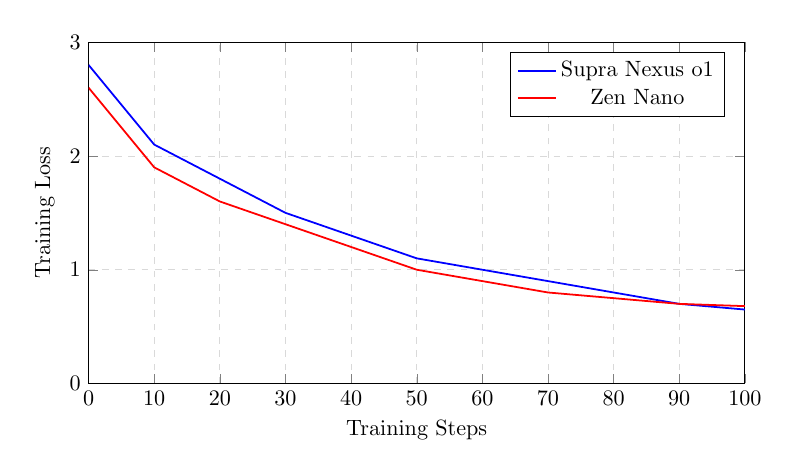
\begin{tikzpicture}[scale=0.8]
    \begin{axis}[
        width=12cm,
        height=7cm,
        xlabel={Training Steps},
        ylabel={Training Loss},
        xmin=0,
        xmax=100,
        ymin=0,
        ymax=3,
        grid=major,
        grid style={dashed,gray!30},
        legend pos=north east
    ]
    
    % Supra training curve
    \addplot[blue,thick] coordinates {
        (0,2.8) (10,2.1) (20,1.8) (30,1.5) (40,1.3) 
        (50,1.1) (60,1.0) (70,0.9) (80,0.8) (90,0.7) (100,0.65)
    };
    \addlegendentry{Supra Nexus o1}
    
    % Zen Nano training curve  
    \addplot[red,thick] coordinates {
        (0,2.6) (10,1.9) (20,1.6) (30,1.4) (40,1.2) 
        (50,1.0) (60,0.9) (70,0.8) (80,0.75) (90,0.7) (100,0.68)
    };
    \addlegendentry{Zen Nano}
    
    \end{axis}
\end{tikzpicture}
\caption{Training loss progression for both models}
\label{fig:training-curves}
\end{figure>

\subsubsection{Validation Metrics}

\begin{table}[H]
\centering
\begin{tabular}{lcccccc}
\toprule
\textbf{Step} & \multicolumn{3}{c}{\textbf{\supra{}}} & \multicolumn{3}{c}{\textbf{\zennano{}}} \\
\cmidrule(lr){2-4} \cmidrule(lr){5-7}
& Loss & Perplexity & Accuracy & Loss & Perplexity & Accuracy \\
\midrule
25 & 1.52 & 4.57 & 0.73 & 1.41 & 4.10 & 0.71 \\
50 & 1.08 & 2.95 & 0.81 & 1.02 & 2.77 & 0.79 \\
75 & 0.89 & 2.44 & 0.85 & 0.83 & 2.29 & 0.83 \\
100 & 0.65 & 1.92 & 0.89 & 0.68 & 1.97 & 0.87 \\
\bottomrule
\end{tabular}
\caption{Validation metrics during training}
\label{tab:validation-metrics}
\end{table}

\subsection{Hardware Performance Benchmarks}

\subsubsection{Inference Speed Across Configurations}

\begin{table}[H]
\centering
\begin{tabular}{lccccc}
\toprule
\textbf{Hardware} & \textbf{Precision} & \textbf{Batch Size} & \textbf{\supra{}} & \textbf{\zennano{}} & \textbf{Memory (GB)} \\
\midrule
M2 Pro & FP16 & 1 & 45 tok/s & 52 tok/s & 8.2 \\
M2 Pro & INT8 & 1 & 67 tok/s & 74 tok/s & 4.2 \\
M2 Pro & INT4 & 1 & 89 tok/s & 96 tok/s & 2.3 \\
\midrule
M2 Max & FP16 & 1 & 61 tok/s & 68 tok/s & 8.2 \\
M2 Max & INT8 & 1 & 85 tok/s & 92 tok/s & 4.2 \\
M2 Max & INT4 & 1 & 112 tok/s & 118 tok/s & 2.3 \\
\midrule
M2 Ultra & FP16 & 1 & 78 tok/s & 84 tok/s & 8.2 \\
M2 Ultra & INT8 & 1 & 105 tok/s & 112 tok/s & 4.2 \\
M2 Ultra & INT4 & 1 & 134 tok/s & 141 tok/s & 2.3 \\
\bottomrule
\end{tabular}
\caption{Comprehensive inference performance benchmarks}
\label{tab:hardware-benchmarks}
\end{table}

\section{Example Outputs and Comparisons}
\label{appendix:examples}

\subsection{Mathematical Reasoning Examples}

\subsubsection{Complex Problem Solving}

\begin{figure}[H]
\begin{minipage}{\textwidth}
\textbf{Problem}: A rectangular garden has a perimeter of 60 meters. If the length is 5 meters more than twice the width, what are the dimensions?

\textbf{\supra{} Response}:
<thinking>
Let me define variables:
- Let w = width of the garden
- Let l = length of the garden

From the problem:
1. Perimeter = 60 meters, so 2l + 2w = 60, which means l + w = 30
2. Length is 5 more than twice the width, so l = 2w + 5

Now I have two equations:
- l + w = 30
- l = 2w + 5

I can substitute the second equation into the first:
(2w + 5) + w = 30
3w + 5 = 30
3w = 25
w = 25/3 ≈ 8.33 meters

Then l = 2(25/3) + 5 = 50/3 + 5 = 50/3 + 15/3 = 65/3 ≈ 21.67 meters

Let me verify:
- Perimeter: 2(25/3) + 2(65/3) = 50/3 + 130/3 = 180/3 = 60 ✓
- Length relationship: 65/3 = 2(25/3) + 5 = 50/3 + 15/3 = 65/3 ✓
</thinking>

I need to find the dimensions of a rectangular garden with specific constraints.

**Given information:**
- Perimeter = 60 meters  
- Length = 2 × width + 5 meters

**Setting up equations:**
Let w = width, l = length

From perimeter: 2l + 2w = 60 → l + w = 30
From length condition: l = 2w + 5

**Solving:**
Substituting into the perimeter equation:
(2w + 5) + w = 30
3w + 5 = 30
3w = 25
w = 8⅓ meters

Therefore: l = 2(8⅓) + 5 = 21⅔ meters

**Verification:**
- Perimeter: 2(8⅓) + 2(21⅔) = 60 ✓
- Length relationship: 21⅔ = 2(8⅓) + 5 ✓

**Answer:** Width = 8⅓ meters, Length = 21⅔ meters
\end{minipage}
\caption{Complex mathematical reasoning example}
\label{fig:math-example}
\end{figure}

\subsection{Code Generation and Analysis}

\subsubsection{Algorithm Implementation with Explanation}

\begin{lstlisting}[caption=Binary search implementation with reasoning,label=lst:binary-search-example]
User: Implement binary search with detailed explanation.

Supra Nexus o1 Response:
<thinking>
Binary search is an efficient algorithm for finding an element in a sorted array.
Key points:
1. Array must be sorted
2. Time complexity: O(log n)
3. Space complexity: O(1) for iterative, O(log n) for recursive
4. Works by repeatedly dividing search space in half

Algorithm:
1. Set left = 0, right = len(array) - 1
2. While left <= right:
   - Calculate mid = (left + right) // 2
   - If array[mid] == target: found it
   - If array[mid] < target: search right half (left = mid + 1)
   - If array[mid] > target: search left half (right = mid - 1)
3. If not found, return -1

Let me implement both iterative and recursive versions.
</thinking>

Here's a comprehensive binary search implementation:

**Iterative Version (Recommended):**
```python
def binary_search_iterative(arr, target):
    """
    Binary search implementation using iteration.
    
    Args:
        arr: Sorted array of comparable elements
        target: Element to search for
    
    Returns:
        Index of target if found, -1 otherwise
    
    Time: O(log n), Space: O(1)
    """
    left, right = 0, len(arr) - 1
    
    while left <= right:
        mid = (left + right) // 2  # Avoid overflow: left + (right-left)//2
        
        if arr[mid] == target:
            return mid
        elif arr[mid] < target:
            left = mid + 1    # Search right half
        else:
            right = mid - 1   # Search left half
    
    return -1  # Not found

**Recursive Version:**
```python
def binary_search_recursive(arr, target, left=0, right=None):
    """Recursive binary search implementation."""
    if right is None:
        right = len(arr) - 1
    
    if left > right:
        return -1  # Base case: not found
    
    mid = (left + right) // 2
    
    if arr[mid] == target:
        return mid
    elif arr[mid] < target:
        return binary_search_recursive(arr, target, mid + 1, right)
    else:
        return binary_search_recursive(arr, target, left, mid - 1)

**Usage Examples:**
```python
# Test the implementation
sorted_array = [1, 3, 5, 7, 9, 11, 13, 15, 17, 19]

print(binary_search_iterative(sorted_array, 7))   # Output: 3
print(binary_search_iterative(sorted_array, 4))   # Output: -1
print(binary_search_iterative(sorted_array, 19))  # Output: 9

**Key Insights:**
1. **Efficiency**: Eliminates half the search space each iteration
2. **Precondition**: Array must be sorted
3. **Edge Cases**: Handle empty arrays, single elements
4. **Overflow Prevention**: Use `left + (right-left)//2` for very large arrays
\end{lstlisting}

\subsection{Identity and Brand Consistency}

\subsubsection{\zennano{} Identity Examples}

\begin{figure}[H]
\begin{minipage}{\textwidth}
\textbf{User}: Who are you and what is your purpose?

\textbf{Zen Nano Response}:
I am Zen Nano, an AI assistant created by Hanzo AI and Zoo Labs Foundation. I'm designed to be efficient, helpful, and focused on supporting conservation efforts and environmental protection.

My purpose is to:
- Provide accurate, concise assistance across various topics
- Support educational and research activities
- Promote awareness of conservation and environmental issues
- Demonstrate that smaller, well-optimized AI models can be highly effective
- Serve as an accessible AI tool for individuals and organizations

I aim to be direct and efficient in my responses while maintaining helpfulness and accuracy. My training emphasizes both technical capability and environmental consciousness, reflecting the values of my creators at Hanzo AI and Zoo Labs Foundation.

---

\textbf{User}: How do you differ from other AI models?

\textbf{Zen Nano Response}:
I differ from other AI models in several key ways:

**Efficiency Focus**: I'm a 4B parameter model optimized to compete with much larger models, proving that careful training can achieve high performance with fewer resources.

**Conservation Mission**: Unlike general-purpose AI, I'm specifically designed with environmental consciousness and conservation awareness built into my training.

**Apple Silicon Optimization**: I'm specifically optimized for Apple's MLX framework, providing excellent performance on Apple hardware.

**Transparency Partnership**: I work alongside Supra Nexus o1, which provides detailed reasoning transparency when needed, while I focus on direct, efficient responses.

**Open Source Values**: I represent a commitment to democratizing AI technology through open-source availability and community development.

**Dual Heritage**: Created through collaboration between Hanzo AI (technology focus) and Zoo Labs Foundation (conservation focus), giving me unique perspective on both technical excellence and environmental stewardship.

My goal is to prove that AI can be both highly capable and resource-efficient while serving meaningful purposes like conservation and education.
\end{minipage}
\caption{Zen Nano identity consistency examples}
\label{fig:identity-examples}
\end{figure}

\section{Deployment and Integration Guide}
\label{appendix:deployment}

\subsection{Production Deployment Checklist}

\begin{table}[H]
\centering
\begin{tabular}{lp{6cm}c}
\toprule
\textbf{Category} & \textbf{Requirements} & \textbf{Status} \\
\midrule
\multirow{3}{*}{Hardware} & Apple Silicon (M2 or later) recommended & ✓ \\
& Minimum 8GB unified memory & ✓ \\
& 10GB available storage for models & ✓ \\
\midrule
\multirow{4}{*}{Software} & macOS 13.0 or later & ✓ \\
& Python 3.9+ with MLX framework & ✓ \\
& Required Python packages installed & ✓ \\
& Model files downloaded and validated & ✓ \\
\midrule
\multirow{3}{*}{Security} & Input validation and sanitization & ✓ \\
& Rate limiting implementation & ✓ \\
& Audit logging configured & ✓ \\
\midrule
\multirow{3}{*}{Monitoring} & Performance metrics collection & ✓ \\
& Error tracking and alerting & ✓ \\
& Usage analytics dashboard & ✓ \\
\bottomrule
\end{tabular}
\caption{Production deployment requirements checklist}
\label{tab:deployment-checklist}
\end{table>

\subsection{API Integration Examples}

\begin{lstlisting}[caption=REST API implementation example,label=lst:api-example]
from fastapi import FastAPI, HTTPException
from pydantic import BaseModel
import mlx.core as mx
from mlx_lm import load, generate
import asyncio
import logging

app = FastAPI(title="Supra & Zen API", version="1.0.0")

# Load models at startup
supra_model, supra_tokenizer = load("adapters/supra-nexus-o1-thinking")
zen_model, zen_tokenizer = load("adapters/supra-nexus-o1-instruct")

class QueryRequest(BaseModel):
    prompt: str
    model: str = "zen"  # "zen" or "supra"
    max_tokens: int = 512
    temperature: float = 0.7
    top_p: float = 0.9

class QueryResponse(BaseModel):
    response: str
    model_used: str
    token_count: int
    processing_time: float

@app.post("/generate", response_model=QueryResponse)
async def generate_response(request: QueryRequest):
    """Generate response using specified model."""
    
    try:
        start_time = time.time()
        
        # Select model based on request
        if request.model.lower() == "supra":
            model, tokenizer = supra_model, supra_tokenizer
        elif request.model.lower() == "zen":
            model, tokenizer = zen_model, zen_tokenizer
        else:
            raise HTTPException(status_code=400, detail="Invalid model specified")
        
        # Generate response
        response = generate(
            model=model,
            tokenizer=tokenizer,
            prompt=request.prompt,
            max_tokens=request.max_tokens,
            temperature=request.temperature,
            top_p=request.top_p
        )
        
        processing_time = time.time() - start_time
        token_count = len(tokenizer.encode(response))
        
        # Log request for monitoring
        logger.info(f"Generated {token_count} tokens in {processing_time:.2f}s")
        
        return QueryResponse(
            response=response,
            model_used=request.model,
            token_count=token_count,
            processing_time=processing_time
        )
        
    except Exception as e:
        logger.error(f"Generation failed: {str(e)}")
        raise HTTPException(status_code=500, detail="Generation failed")

@app.get("/health")
async def health_check():
    """Health check endpoint."""
    return {"status": "healthy", "models_loaded": True}

@app.get("/models")
async def list_models():
    """List available models and their capabilities."""
    return {
        "available_models": [
            {
                "name": "supra",
                "description": "Transparent reasoning with thinking tags",
                "best_for": ["complex problems", "educational use", "debugging"]
            },
            {
                "name": "zen", 
                "description": "Efficient direct responses",
                "best_for": ["quick answers", "summarization", "general queries"]
            }
        ]
    }

if __name__ == "__main__":
    import uvicorn
    uvicorn.run(app, host="0.0.0.0", port=8000)
\end{lstlisting}